\documentclass[]{article}
\usepackage{graphicx}
\graphicspath{ {../print/} }
%opening
\title{Catchment Level Predictive Mapping of 535 Fish Species Distributions}
\author{Douglas Patton}

\begin{document}

\maketitle

\begin{abstract}
Using an existing dataset of wadeable freshwater stream fish inventories, we apply statistical learning techniques to produce predictive distributions for the Continental United States (CONUS). We use around *400* of the catchment-level metrics in the StreamCat dataset as predictors. We created classification machine learning pipelines with both linear and non-linear statistical learners and we estimated both full-data classification models and probabilistic models. To communicate modeling uncertainty, we also use the cross-validation results to generate maps showing prediction intervals.  To quantify the uncertainty of our predictive models
\end{abstract}

\section{Introduction}
In order to provide the public with enhanced fish distribution maps and predictive mapping tools, we apply machine learning classification modeling to create predictive maps using an existing dataset of electrofishing inventories spanning much of the Contiguous United States (CONUS).  

\section{Methods}
\subsection{Data}
We utilize the dataset of electrofishing inventories from cite{cyterski2000} to create a binary dataset of catchments labeled for each species as present if the species had been found there at least once and absent otherwise. In comparison to cite{cyterski2000}, who defined occurrence as a species appearing in the majority of visits, our approach will create a dataset with a greater share of species occurrences rather than absences for sites visited more than one time. 
Across the species in our dataset, the distribution and relationship between sample size and the average occurrence rate, $\bar{y}$, can be seen in \ref{fig:hist_n_y} and \ref{fig:scatter_n_y}. The lower left half of \ref{fig:scatter_n_y} is empty due to the lower limit on detecting a species with low occurrence rates for a given sample size, $\bar{y}_{min}=1/N$.
The predictor covariates for each species come entirely from the EPA StreamCat database. This database contains over 400 catchment level metrics that describe both the surround catchment of flowing waters and teh cumulative, upstream watershed. We exclude a small number of repetitive metrics such as early iterations of complex multi-input metrics and dam/reservoir metrics with similar information

\subsection{Modeling}
The foundation of our classification modeling is the scikit-learn cite{pedregosa} pipeline. This tool is useful for encapsulating estimation code, allowing for repeated application of a multi-step algorithm across species and during re-sampling. Each of the pipelines that we develop contains an imputation step that implements the K nearest neighbors algorithm (K=5) and is followed by an estimation step that implements the main statistical learner. We also include a linear regression pipeline that converts the regression prediction into a classification problem with a decision threshold at 0.5. Classification algorithms included are gradient boosting classifier, histogram gradient boosting classifier, linear and RBF kernel support vector machines, and regularized logistic regression.


\section{Results}
The first set of our results is a basic overview of modeling performance across geographies
To provide an overview of modeling performance and aggregate fish distributions, we created a confusion matrix \ref{fig:y01}


\begin{figure}
	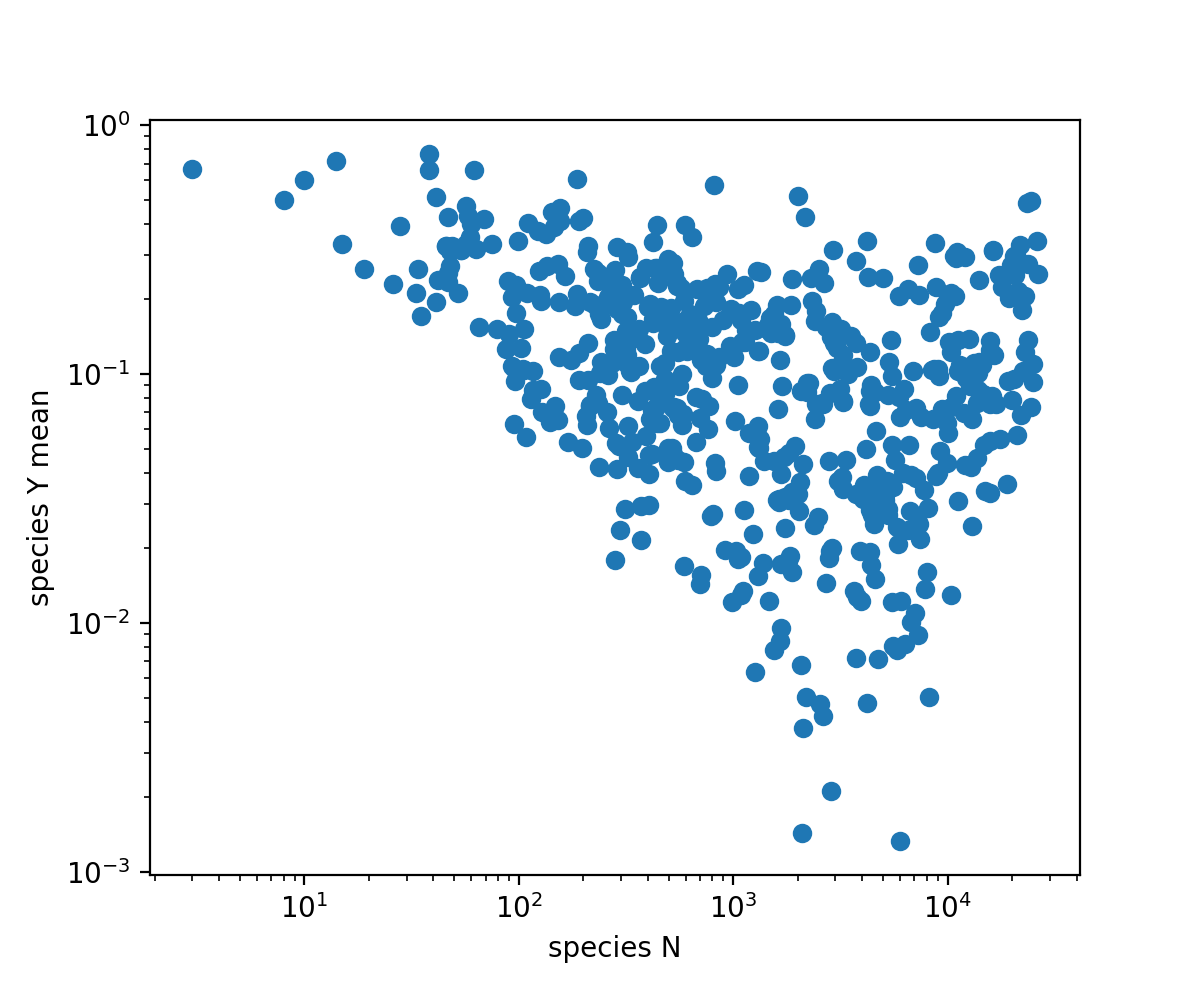
\includegraphics[width=\linewidth]{xy_scatter_log.png}
	\caption{A scatter plot of species sample size on the horizontal axis and species average occurrence rate on the vertical axis}
	\label{fig:scatter_n_y}
\end{figure}

\begin{figure}
	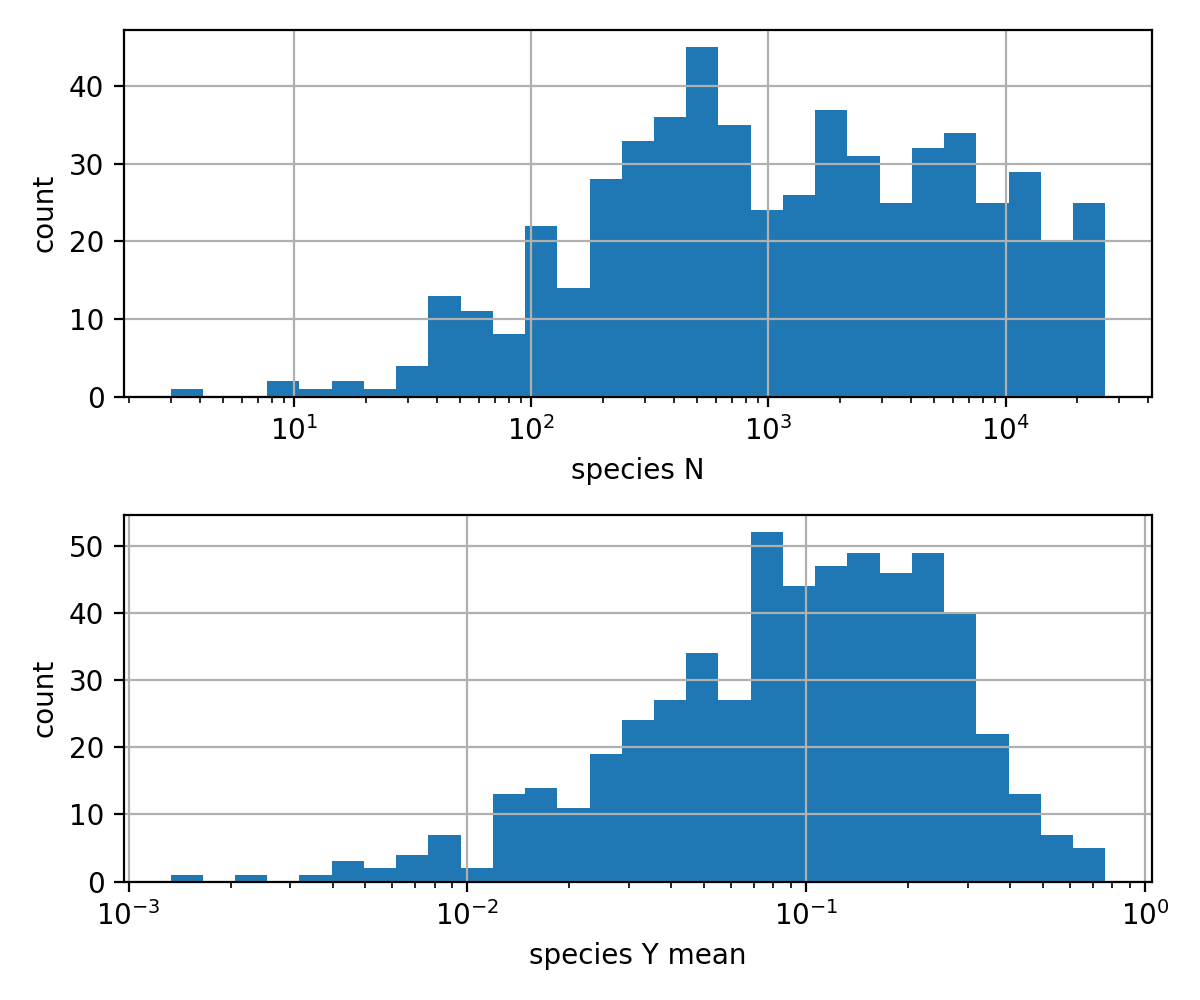
\includegraphics[width=\linewidth]{basic_histogram_log.png}
	\caption{A histogram of  each species sample size and each species mean occurrence rate}
	\label{fig:hist_n_y}
\end{figure}


\begin{figure}
	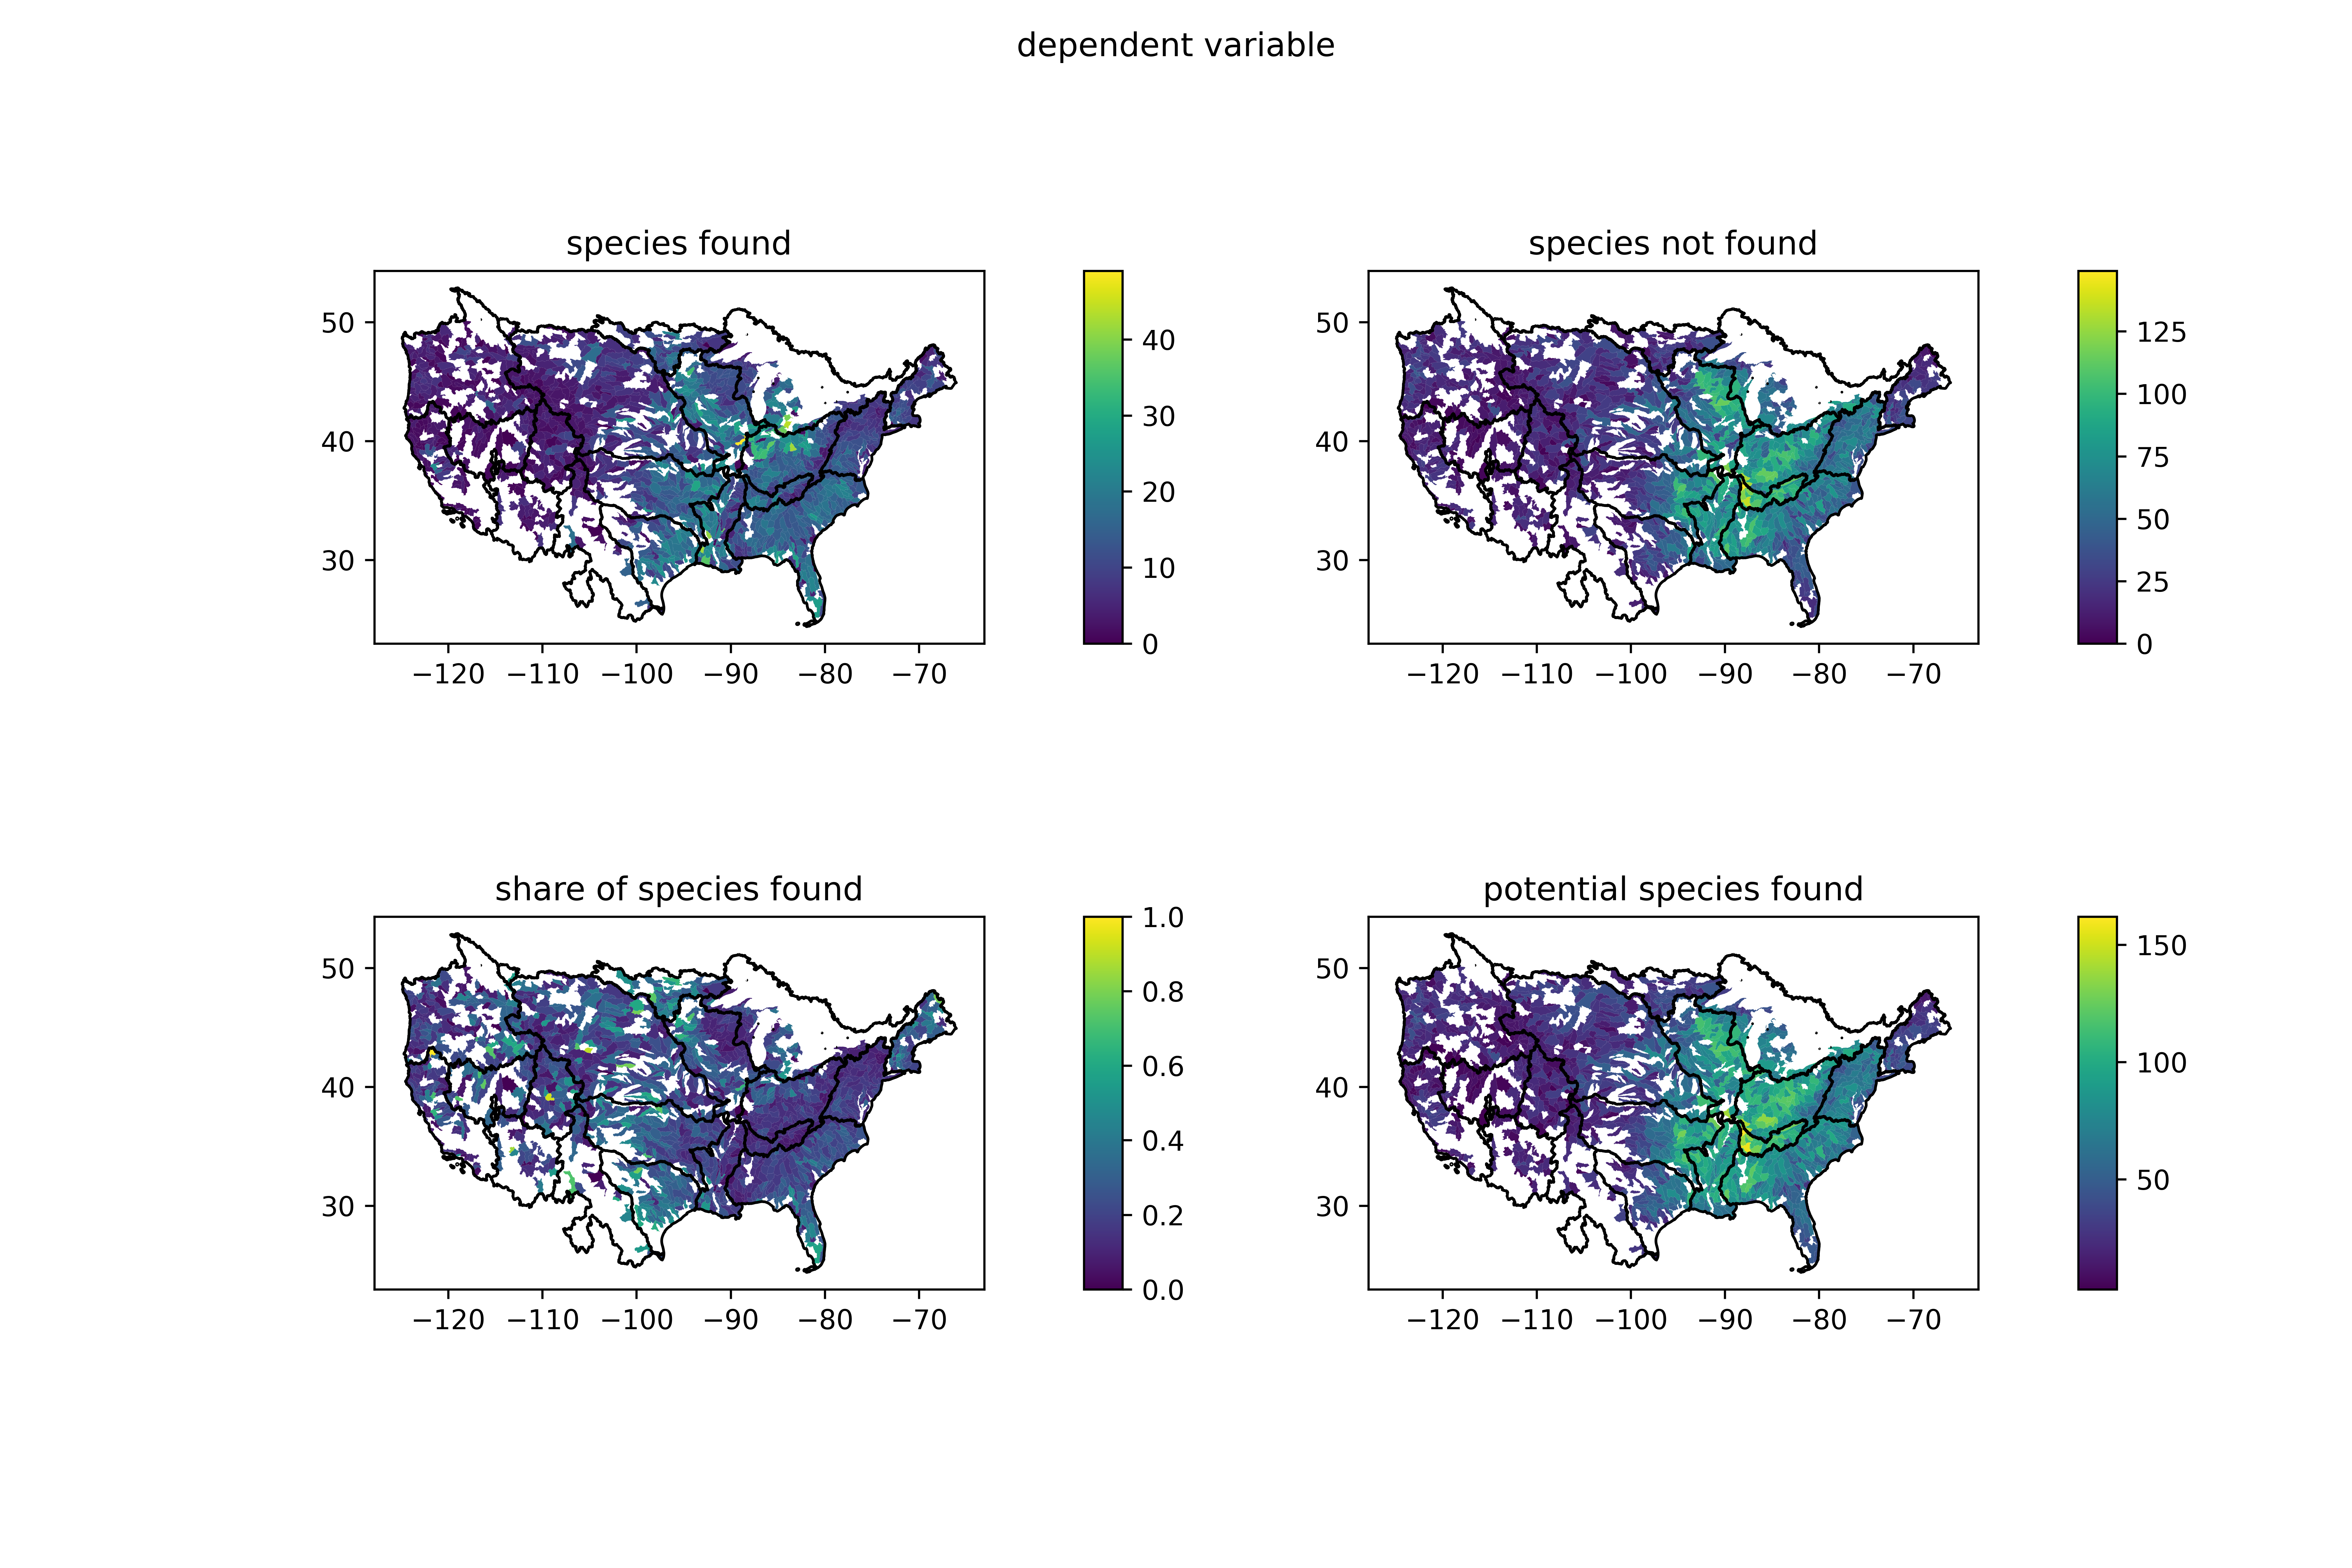
\includegraphics[width=\linewidth]{y01_huc8.png}
	\caption{A confusion matrix map with average metrics across comids in each HUC8}
	\label{fig:y01}
\end{figure}

\end{document}



